% Template for PLoS
% Version 3.6 Aug 2022
%
% % % % % % % % % % % % % % % % % % % % % %
%
% -- IMPORTANT NOTE
%
% This template contains comments intended 
% to minimize problems and delays during our production 
% process. Please follow the template instructions
% whenever possible.
%
% % % % % % % % % % % % % % % % % % % % % % % 
%
% Once your paper is accepted for publication, 
% PLEASE REMOVE ALL TRACKED CHANGES in this file 
% and leave only the final text of your manuscript. 
% PLOS recommends the use of latexdiff to track changes during review, as this will help to maintain a clean tex file.
% Visit https://www.ctan.org/pkg/latexdiff?lang=en for info or contact us at latex@plos.org.
%
%
% There are no restrictions on package use within the LaTeX files except that no packages listed in the template may be deleted.
%
% Please do not include colors or graphics in the text.
%
% The manuscript LaTeX source should be contained within a single file (do not use \input, \externaldocument, or similar commands).
%
% % % % % % % % % % % % % % % % % % % % % % %
%
% -- FIGURES AND TABLES
%
% Please include tables/figure captions directly after the paragraph where they are first cited in the text.
%
% DO NOT INCLUDE GRAPHICS IN YOUR MANUSCRIPT
% - Figures should be uploaded separately from your manuscript file. 
% - Figures generated using LaTeX should be extracted and removed from the PDF before submission. 
% - Figures containing multiple panels/subfigures must be combined into one image file before submission.
% For figure citations, please use "Fig" instead of "Figure".
% See http://journals.plos.org/plosone/s/figures for PLOS figure guidelines.
%
% Tables should be cell-based and may not contain:
% - spacing/line breaks within cells to alter layout or alignment
% - do not nest tabular environments (no tabular environments within tabular environments)
% - no graphics or colored text (cell background color/shading OK)
% See http://journals.plos.org/plosone/s/tables for table guidelines.
%
% For tables that exceed the width of the text column, use the adjustwidth environment as illustrated in the example table in text below.
%
% % % % % % % % % % % % % % % % % % % % % % % %
%
% -- EQUATIONS, MATH SYMBOLS, SUBSCRIPTS, AND SUPERSCRIPTS
%
% IMPORTANT
% Below are a few tips to help format your equations and other special characters according to our specifications. For more tips to help reduce the possibility of formatting errors during conversion, please see our LaTeX guidelines at http://journals.plos.org/plosone/s/latex
%
% For inline equations, please be sure to include all portions of an equation in the math environment.  For example, x$^2$ is incorrect; this should be formatted as $x^2$ (or $\mathrm{x}^2$ if the romanized font is desired).
%
% Do not include text that is not math in the math environment. For example, CO2 should be written as CO\textsubscript{2} instead of CO$_2$.
%
% Please add line breaks to long display equations when possible in order to fit size of the column. 
%
% For inline equations, please do not include punctuation (commas, etc) within the math environment unless this is part of the equation.
%
% When adding superscript or subscripts outside of brackets/braces, please group using {}.  For example, change "[U(D,E,\gamma)]^2" to "{[U(D,E,\gamma)]}^2". 
%
% Do not use \cal for caligraphic font.  Instead, use \mathcal{}
%
% % % % % % % % % % % % % % % % % % % % % % % % 
%
% Please contact latex@plos.org with any questions.
%
% % % % % % % % % % % % % % % % % % % % % % % %

\documentclass[10pt,letterpaper]{article}
\usepackage[top=0.85in,left=2.75in,footskip=0.75in]{geometry}

% amsmath and amssymb packages, useful for mathematical formulas and symbols
\usepackage{amsmath,amssymb}

% Use adjustwidth environment to exceed column width (see example table in text)
\usepackage{changepage}

% textcomp package and marvosym package for additional characters
\usepackage{textcomp,marvosym}

% cite package, to clean up citations in the main text. Do not remove.
\usepackage{cite}

% Use nameref to cite supporting information files (see Supporting Information section for more info)
\usepackage{nameref,hyperref}

% line numbers
\usepackage[right]{lineno}

% ligatures disabled
\usepackage[nopatch=eqnum]{microtype}
\DisableLigatures[f]{encoding = *, family = * }

% color can be used to apply background shading to table cells only
\usepackage[table]{xcolor}

% array package and thick rules for tables
\usepackage{array}

% create "+" rule type for thick vertical lines
\newcolumntype{+}{!{\vrule width 2pt}}

% create \thickcline for thick horizontal lines of variable length
\newlength\savedwidth
\newcommand\thickcline[1]{%
  \noalign{\global\savedwidth\arrayrulewidth\global\arrayrulewidth 2pt}%
  \cline{#1}%
  \noalign{\vskip\arrayrulewidth}%
  \noalign{\global\arrayrulewidth\savedwidth}%
}

% \thickhline command for thick horizontal lines that span the table
\newcommand\thickhline{\noalign{\global\savedwidth\arrayrulewidth\global\arrayrulewidth 2pt}%
\hline
\noalign{\global\arrayrulewidth\savedwidth}}


% Remove comment for double spacing
%\usepackage{setspace} 
%\doublespacing

% Text layout
\raggedright
\setlength{\parindent}{0.5cm}
\textwidth 5.25in 
\textheight 8.75in

% Bold the 'Figure #' in the caption and separate it from the title/caption with a period
% Captions will be left justified
\usepackage[aboveskip=1pt,labelfont=bf,labelsep=period,justification=raggedright,singlelinecheck=off]{caption}
\renewcommand{\figurename}{Fig}

% Use the PLoS provided BiBTeX style
\bibliographystyle{plos2015}

% Remove brackets from numbering in List of References
\makeatletter
\renewcommand{\@biblabel}[1]{\quad#1.}
\makeatother



% Header and Footer with logo
\usepackage{lastpage,fancyhdr,graphicx}
\usepackage{epstopdf}
%\pagestyle{myheadings}
\pagestyle{fancy}
\fancyhf{}
%\setlength{\headheight}{27.023pt}
%\lhead{\includegraphics[width=2.0in]{PLOS-submission.eps}}
\rfoot{\thepage/\pageref{LastPage}}
\renewcommand{\headrulewidth}{0pt}
\renewcommand{\footrule}{\hrule height 2pt \vspace{2mm}}
\fancyheadoffset[L]{2.25in}
\fancyfootoffset[L]{2.25in}
\lfoot{\today}

%% Include all macros below

\newcommand{\lorem}{{\bf LOREM}}
\newcommand{\ipsum}{{\bf IPSUM}}
\newcommand{\dmc}{\(DMC_x^2\) }
\newcommand{\pdcca}{\({\rho}_{DCCA}\) }
\newcommand{\fdfa}{\(F_{DFA}\) }


%% END MACROS SECTION


\begin{document}
\vspace*{0.2in}

% Title must be 250 characters or less.
\begin{flushleft}
{\Large
\textbf\newline{A \dmc Multi-channel cross-correlation analyses of a motor/imaginary human activity experiment electroencephalogram (EEG) recordings} % Please use "sentence case" for title and headings (capitalize only the first word in a title (or heading), the first word in a subtitle (or subheading), and any proper nouns).
}
\newline
% Insert author names, affiliations and corresponding author email (do not include titles, positions, or degrees).
\\
Fernando Ferraz Ribeiro\textsuperscript{1,4\Yinyang},
Andrea de Almeida Brito\textsuperscript{3\Yinyang},
Florêncio Mendes Oliveira Filho\textsuperscript{5\textcurrency},
Juan Alberto Leyva Cruz\textsuperscript{2},
Gilney Figueira Zebende\textsuperscript{2}
\\
\bigskip
\textbf{1} Federal University of Bahia, Brazil
\\
\textbf{2} State University of Feira de Santana, Bahia, Brazil
\\
\textbf{3} Department of Mathematic, Federal Institute of Education, Science and Techinology , Salvador, Bahia, Brazil 
\\
\textbf{4} PPGM, State University of Feira de Santana, Bahia, Brazil
\\
\textbf{5} Computation Engeneering, SENAI CIMATEC University Center, Salvador, Bahia, Brazil
\bigskip

% Insert additional author notes using the symbols described below. Insert symbol callouts after author names as necessary.
% 
% Remove or comment out the author notes below if they aren't used.
%
% Primary Equal Contribution Note
\Yinyang These authors contributed equally to this work.

% Additional Equal Contribution Note
% Also use this double-dagger symbol for special authorship notes, such as senior authorship.
\ddag These authors also contributed equally to this work.

% Current address notes
\textcurrency Current Address: Dept/Program/Center, Institution Name, City, State, Country % change symbol to "\textcurrency a" if more than one current address note
% \textcurrency b Insert second current address 
% \textcurrency c Insert third current address

% Deceased author note
\dag Deceased

% Group/Consortium Author Note
\textpilcrow Membership list can be found in the Acknowledgments section.

% Use the asterisk to denote corresponding authorship and provide email address in note below.
* correspondingauthor@institute.edu

\end{flushleft}
% Please keep the abstract below 300 words
\section*{Abstract}
This paper presents an investigation on the electroencephalogram (EEG) 64-channels recordings of a motor/imaginary experiment, using the detrended multiple cross-correlation coefficient (\dmc). Analyzing data from 4 channels, \(F_{3}32\), \(F_{6}37\) (frontal region of the head) and \(P_{3}49\), \(P_{6}54\) (parietal region of the head), the \dmc was applied to evaluate the correlation among one of the channels with the three others alternately. Analyzing all the motor/imaginary experiments and 108 of the 109 subjects, this research points to a pattern, detected on most of the subjects: Using channel \(F_{3}32\) against the others, the correlation coefficient is higher compared to the other combinations. The reason why some persons don't match that pattern is still an open question.

% Please keep the Author Summary between 150 and 200 words
% Use first person. PLOS ONE authors please skip this step. 
% Author Summary not valid for PLOS ONE submissions.   
% \section*{Author summary}

\linenumbers

% Use "Eq" instead of "Equation" for equation citations.
\section*{Introduction}

The electroencephalogram (EEG) is, in short, a technic that reads electrical signals from the brain activity with the use of sensors placed in the scalp of the patient and makes sense of this data. Impulses are amplified and recorded over time in parallel, generating one time serie for each sensor. The EEG equipment mesures the electric potential difference from each sensor position in relation with a reference sensor, usually placed in the ear lobe. Although the EEG is almost a centenary technic, in recent decades EEG has addressed new problems as brain-triggered neurorehabilitation treatments, experimental psychology or even computational neuroscience, due to it's versatility and accessibility combined with the advances in signal processing~\cite{Biasiucci2019}.

The recordings used are available at the Physionet on-line databank (\url{https:// physionet.org/pn4/eegmmidb/}). The data is originated from a study that perform 14 experiments on a population of 109 subjects, Using 64 electrodes to record the brain signals. The first 2 experiments are baseline references, the subjects where resting with eyes opened end the second with eyes closed (one minute for each). The other four experiments are a combination of two categories with two possible options each \(2 \times 2\ = 4\). In general, the experiments consist of making the subjects react over visual stimulus: a target that appears on a screen. One category is about the target position, one option is a target that will aperar on the left or the right of the screen, in the other,the target will appear on the top or on the bottom of the screen. The second category determines if the subject will actually execute a body action related to the target position (Real) or if the corresponding action will be just imagined (Imaginary) by the subject. The tasks, with duration of two minutes, are described below:

\begin{itemize}
  \item \bf{Task 1}: a target appears on either the left or the right side of the screen. The subject opens and closes the corresponding fist until the target disappears. Then the subject relaxes. (Real (L/R));
  \item \bf{Task 2}: a target appears on either the left or the right side of the screen. The subject \bf{imagines} opening and closing the corresponding fist until the target disappears. Then the subject relaxes. (Imag (L/R));
  \item \bf{Task 3}: a target appears on either the top or the bottom of the screen. The subject opens and closes either both fists (if the target is on top) or both feet (if the target is on the bottom) until the target disappears. Then the subject relaxes. (Real (T/D));
  \item \bf{Task 4}: a target appears on either the top or the bottom of the screen. The subject \bf{imagines} opening and closing either both fists (if the target is on top) or both feet (if the target is on the bottom) until the target disappears. Then the subject relaxes. (Imag (T/D)).
\end{itemize}

Table \ref{table1} presents witch Task is carried in each experiment number. Every subject executes the four tasks three times. Experiments 3, 7 and 11 applies Task 1 to the subjects, experiments 4, 8 and 12, Task 2, experiments 5, 9 and 13, Task 3 and experiments 6, 10 e 14 uses Task 4.

% Place tables after the first paragraph in which they are cited.
\begin{table}[!ht]
  %\begin{adjustwidth}{-2.25in}{0in} % Comment out/remove adjustwidth environment if table fits in text column.
  \centering
  \caption{
  {\bf Experiment x task relation}}

    \begin{tabular}{|l|l|l|l|l|l|l|l|l|l|l|l|l|l|l|}
    \hline
    Experiment n º & 1 & 2 & 3 & 4 & 5 & 6 & 7 & 8 & 9 & 10 & 11 & 12 & 13 & 14 \\ \thickhline
    Baseline 1     & x &   &   &   &   &   &   &   &   &    &    &    &    &    \\ \hline
    Baseline 2     &   & x &   &   &   &   &   &   &   &    &    &    &    &    \\ \hline
    Task 1         &   &   & x &   &   &   & x &   &   &    & x  &    &    &    \\ \hline
    Task 2         &   &   &   & x &   &   &   & x &   &    &    & x  &    &    \\ \hline
    Task 3         &   &   &   &   & x &   &   &   & x &    &    &    & x  &    \\ \hline
    Task 4         &   &   &   &   &   & x &   &   &   & x  &    &    &    & x  \\ \hline
    \end{tabular}

  \begin{flushleft} The experiment and the executed tasks: Two one-minute baseline (eyes open/closed) and three two-minute of four Tasks.
  \end{flushleft}
  \label{table1}
  %\end{adjustwidth}
  \end{table}

The electrodes in all tasks and experiments where located as shown in Figure \ref{fig:cabeca}. The colored circles in Figure \ref{fig:cabeca} correspond to the positions of the electrodes channels whose recordings were used in our analyses: \(F_{3}32\) (blue) and \(F_{6}37\) (yellow), on the frontal region of the head, and \(P_{3}49\) (red) and \(P_{6}54\) (green), on the parietal region of the head.

\begin{figure}[!h]
  \caption{{\bf Electrodes position illustration.}
  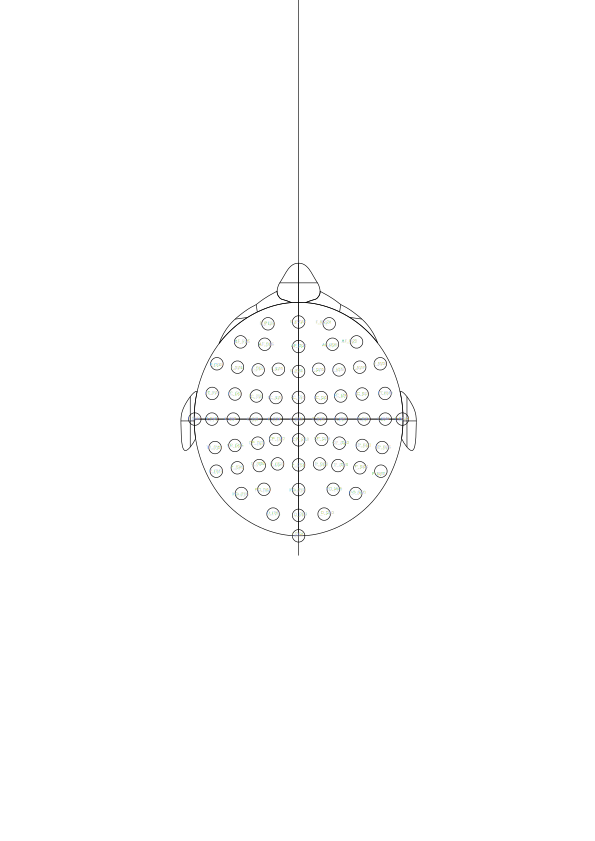
\includegraphics[width=.9\textwidth]{../fig_cabeca/FIG_CABECA.png}
  \\ Position of the 64 electrodes according to the international10-20 system (excluding electrodes Nz, F9, F10, FT9, FT10, A1, A2, TP9, TP10, P9, and P10). The colored dots: \(F_{3}32\) (blue), \(F_{6}37\) (yellow), \(P_{3}49\) (red), \(P_{6}54\) (green) identify the channels used in this research.}
  \label{fig:cabeca}
  \end{figure}

The four channels are alternately picked as dependent variable and the correlation against the other three are calculated by the application of the Detrended Multiple Cross-Correlation Coefficient (\dmc) \cite{Zebende2018}

In the next sections we will present the dataset; the methodology used to analyze the data, including pre-processing strategies and criteria, and the \dmc method; the results, statistics and data visualization for the analyzed populations and individual results for randomly selected subjects. The discussion of the results and the conclusions are presented in sequence. In the supporting materials, a link to access all the calculations and data visualization for all the experiment subjects is available.

\section*{Materials and methods}

The Physionet on-line databank is publicly available at \url{https:// physionet.org/pn4/eegmmidb/}, presents recordings of the EEG experiments described in previous section. The data is  provided in EDF (European data format) files. The files of all the experiments for every subject where downloaded using a web scraping script created by the authors using Python and the package Beautiful Soap.

The EDF files where opened using Python package pyedflib and translated into text files . In EEG experiments, usually the end of the recordings is filled with a sequence of zeroes, corresponding to the time gap between the shooting down of the EEG machine and the recording system. In this pre-processing stage, all the tailing zeroes sequences are eliminated from the records. To properly apply the \dmc calculations and the intended comparisons between experiments end subjects, all the time series must have the same length. The research find out the the	experiment number 5	(Top/Down, Real) conducted with subject S106 has only 5808 valid recorded points. The second smallest time series has 15742 valid records (subject: S100, experiment: 12	-Left/Right,	Imaginary).

The interval between each recorded value in this equipment is 6.25 ms, and the recordings on experiment 5 of subject S106 is 36.3 s. The duration is way smaller then the expected 2 minutes and the series is relatively small to the application os the \dmc method. Cutting all the subjects data to this duration implies in a great loss of data. The second smaller series of 15742 represents a total duration of 98.3875 s. The value was considered adequate to the \dmc method and the duration is about 82\% of the expected duration. The decision was to eliminate subject S106 from the experiment and to cut all time series at recording point 15742. resulting in a total number of 108 subjects with all 12 experiments per subject lasting 98.3875 s.


To analise the dataset, this study uses the Detrended Multiple Cross-Correlation Coefficient (\dmc) \cite{Zebende2018}. This coefficient, based on the \pdcca \cite{Zebende2011}, determinates the correlation between one time serie (as the dependent variable) and a number \(n\) of time series (as independent variables).

The \(DCCA\) aims to identify the existence of a correlations among two time series, and is very similar to the \(DFA\) algorithm: the steps 1, 2 and 3 are calculated for two timeseries \(x_{1i}\) and \(x_{2i}\), generating the integrated series \(X_{1k}\) and \(X_{2k}\) in the first steps and the detrended series \(\widetilde{X}_{1k, i}\) and \(\widetilde{X}_{2k, i}\) in the third step.

\begin{equation} \label{eq:fdcca}
  f_{DCCA}^{2}(n, i) = \frac{1}{1+n} \sum_{k=i}^{i + n} (X_{1k}-\widetilde{X}_{1k, i}) (X_{2k}-\widetilde{X}_{2k, i})
\end{equation}

\begin{equation}\label{eq:dmc_4x_y} 
  \begin{split}
DMC_{x}^{2} \quad = \quad & ( \rho^{2}_{X_{2},X_{3}} \times \rho^{2}_{Y,X_{1}}- \rho^{2}_{Y,X_{1}} + \rho^{2}_{X_{1},X_{3}}\times \rho^{2}_{Y,X_{2}}-\rho^{2}_{Y,X_{2}}+ \\
& 2 \times \rho_{X_{1},X_{2}} \times \rho_{Y,X_{1}} \times \rho_{Y,X_{2}}   - 2 \times \rho_{X_{1},X_{3}} \times \rho_{X_{2},X_{3}} \times \rho_{Y,X_{1}} + \\
& \rho^{2}_{X_{1},X_{2}} \times \rho^{2}_{Y,X_{3}}-\rho^{2}_{Y,X_{3}} + 2 \times \rho_{X_{1},X_{3}} \times \rho_{Y,X_{1}} \times \rho_{Y,X_{3}} - \\ 
& 2 \times \rho_{X_{1},X_{2}} \times \rho_{X_{2},X_{3}} \times \rho_{Y,X_{1}} \times \rho_{Y,X_{3}} - \\
& 2 \times \rho_{X_{1},X_{2}} \times \rho_{X_{1},X_{3}} \times \rho_{Y,X_{2}} \times \rho_{Y,X_{3}} + \\
& 2 \times \rho_{X_{2},X_{3}} \times \rho_{Y,X_{2}} \times \rho_{Y,X_{3}} ) \quad / \\
& ( \rho^{2}_{X_{1},X_{2}} + \rho^{2}_{X_{1},X_{3}} + \rho^{2}_{X_{2},X_{3}} - 2 \times \rho_{X_{1},X_{2}} \times \rho_{X_{1},X_{3}} \times \rho_{X_{2},X_{3}}^{-1}) \\
 \end{split}
\end{equation}

The \fdfa root mean square (rms) fluctuation function was already used to analyze a subset of the same dataset used here to evaluate   \cite{Mesquita2019} \cite{OliveiraFilho2019} \cite{OliveiraFilho2021}


\cite{Peng1994, Buldyrev1950}, \cite{Podobnik2008}, \cite{Zebende2011}, \cite{PhysRevE.84.066118}, 

% \begin{eqnarray}
% \label{eq:schemeP}
% 	\mathrm{P_Y} = \underbrace{H(Y_n) - H(Y_n|\mathbf{V}^{Y}_{n})}_{S_Y} + \underbrace{H(Y_n|\mathbf{V}^{Y}_{n})- H(Y_n|\mathbf{V}^{X,Y}_{n})}_{T_{X\rightarrow Y}},
% \end{eqnarray}

% Results and Discussion can be combined.
\section*{Results}

% For figure citations, please use "Fig" instead of "Figure".
Fig~\ref{fig1} 

% Place figure captions after the first paragraph in which they are cited.
\begin{figure}[!h]
\caption{{\bf Bold the figure title.}
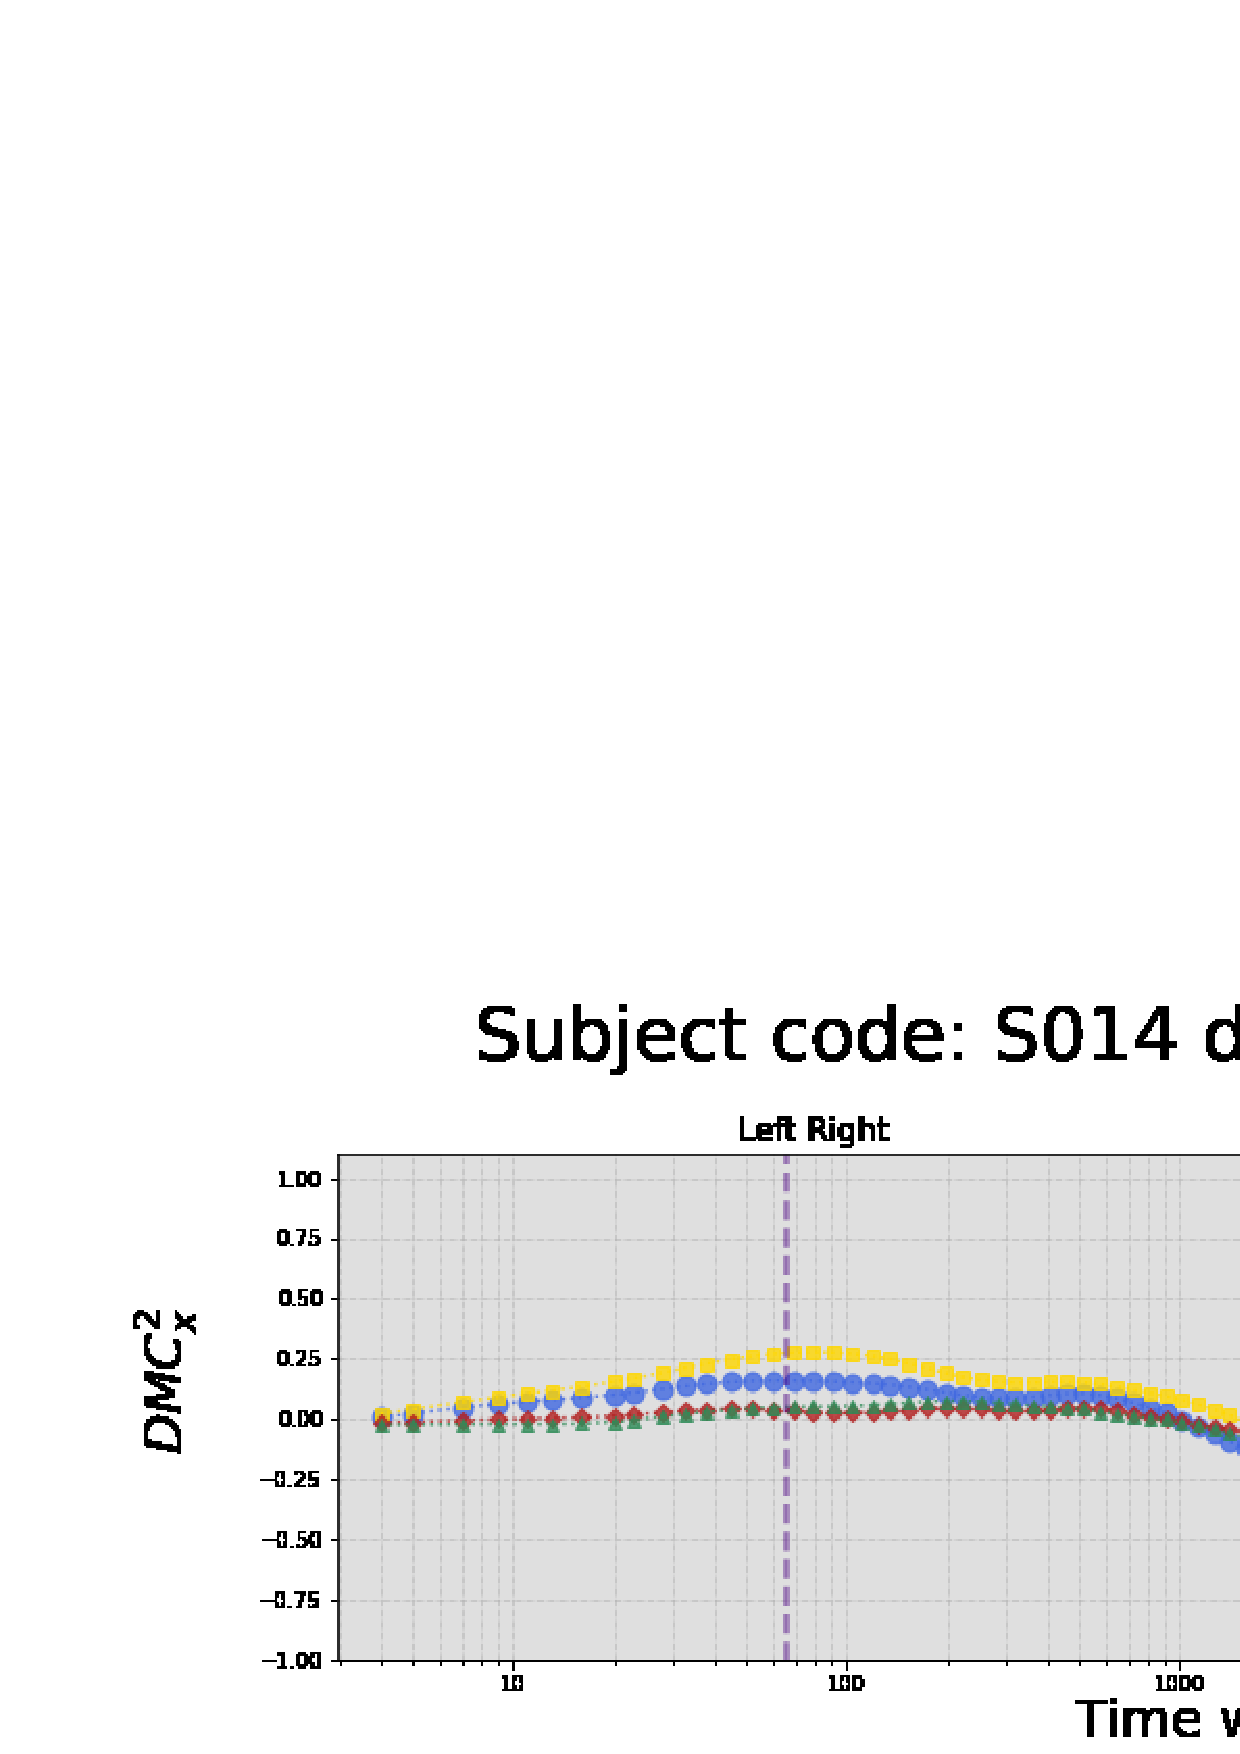
\includegraphics[width=.9\textwidth]{../output/figs/stats/S014.jpg}
Figure caption text here, please use this space for the figure panel descriptions instead of using subfigure commands. A: Lorem ipsum dolor sit amet. B: Consectetur adipiscing elit.}
\label{fig1}
\end{figure}

\begin{figure}[!h]
  \caption{{\bf Bold the figure title.}
  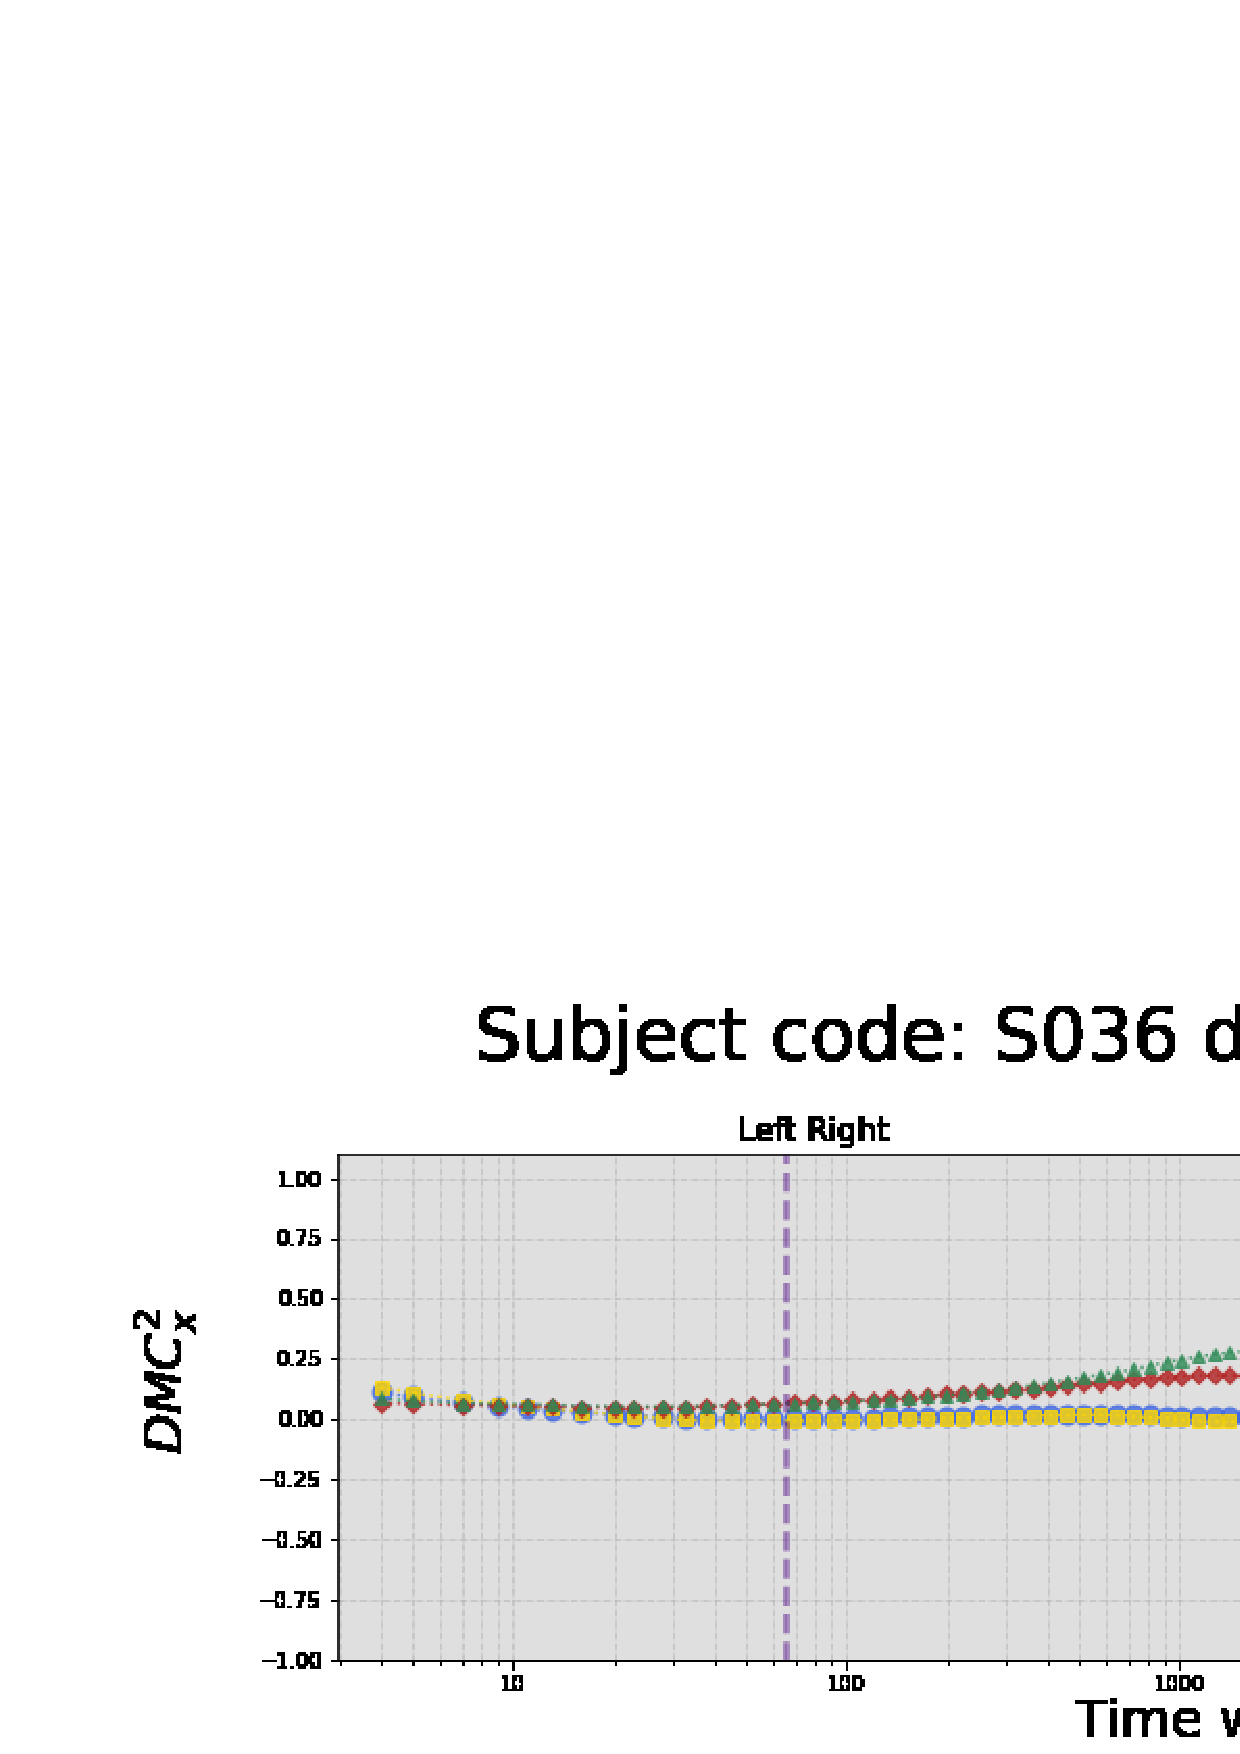
\includegraphics[width=.9\textwidth]{../output/figs/stats/S036.jpg}
  Figure caption text here, please use this space for the figure panel descriptions instead of using subfigure commands. A: Lorem ipsum dolor sit amet. B: Consectetur adipiscing elit.}
  \label{fig36}
\end{figure}

\begin{figure}[!h]
    \caption{{\bf Bold the figure title.}
    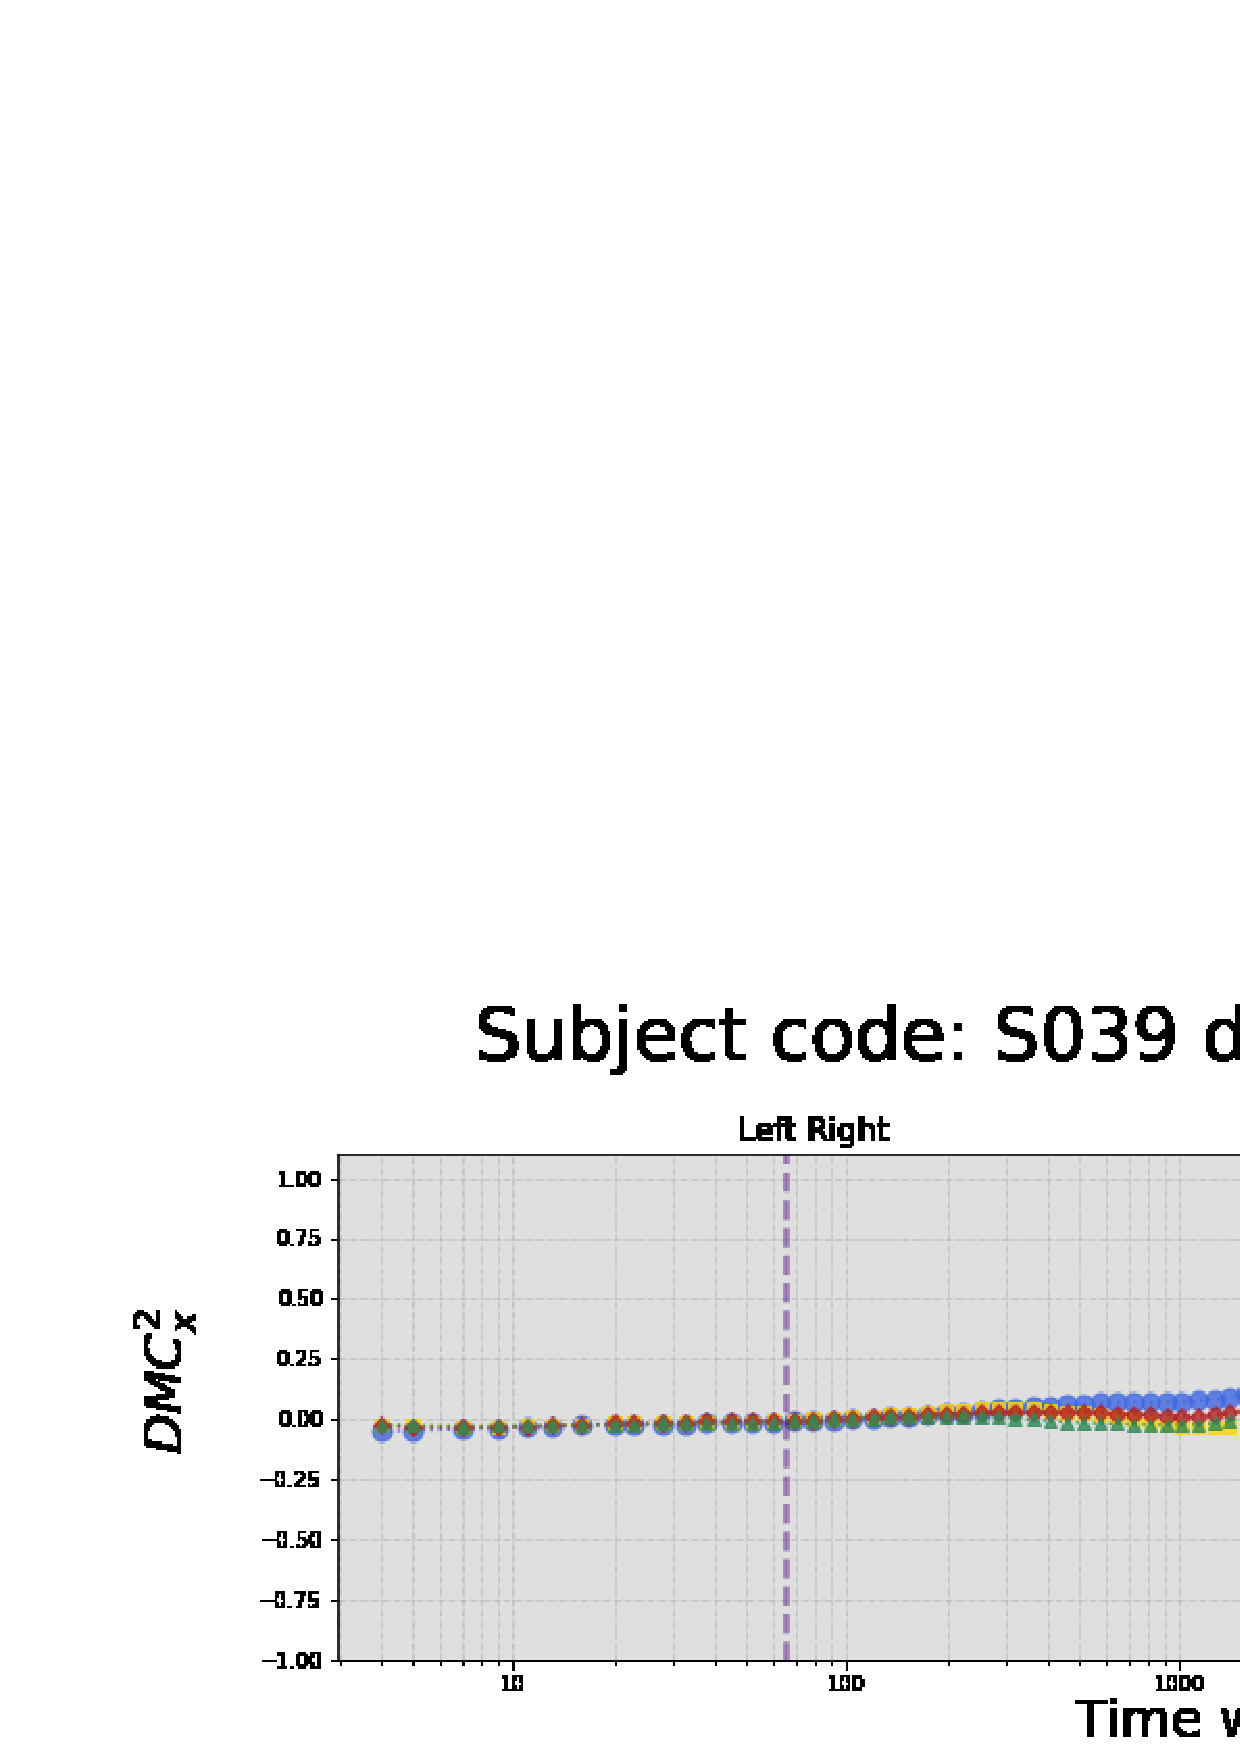
\includegraphics[width=.9\textwidth]{../output/figs/stats/S039.jpg}
    Figure caption text here, please use this space for the figure panel descriptions instead of using subfigure commands. A: Lorem ipsum dolor sit amet. B: Consectetur adipiscing elit.}
    \label{fig39}
\end{figure}

\begin{figure}[!h]
    \caption{{\bf Bold the figure title.}
    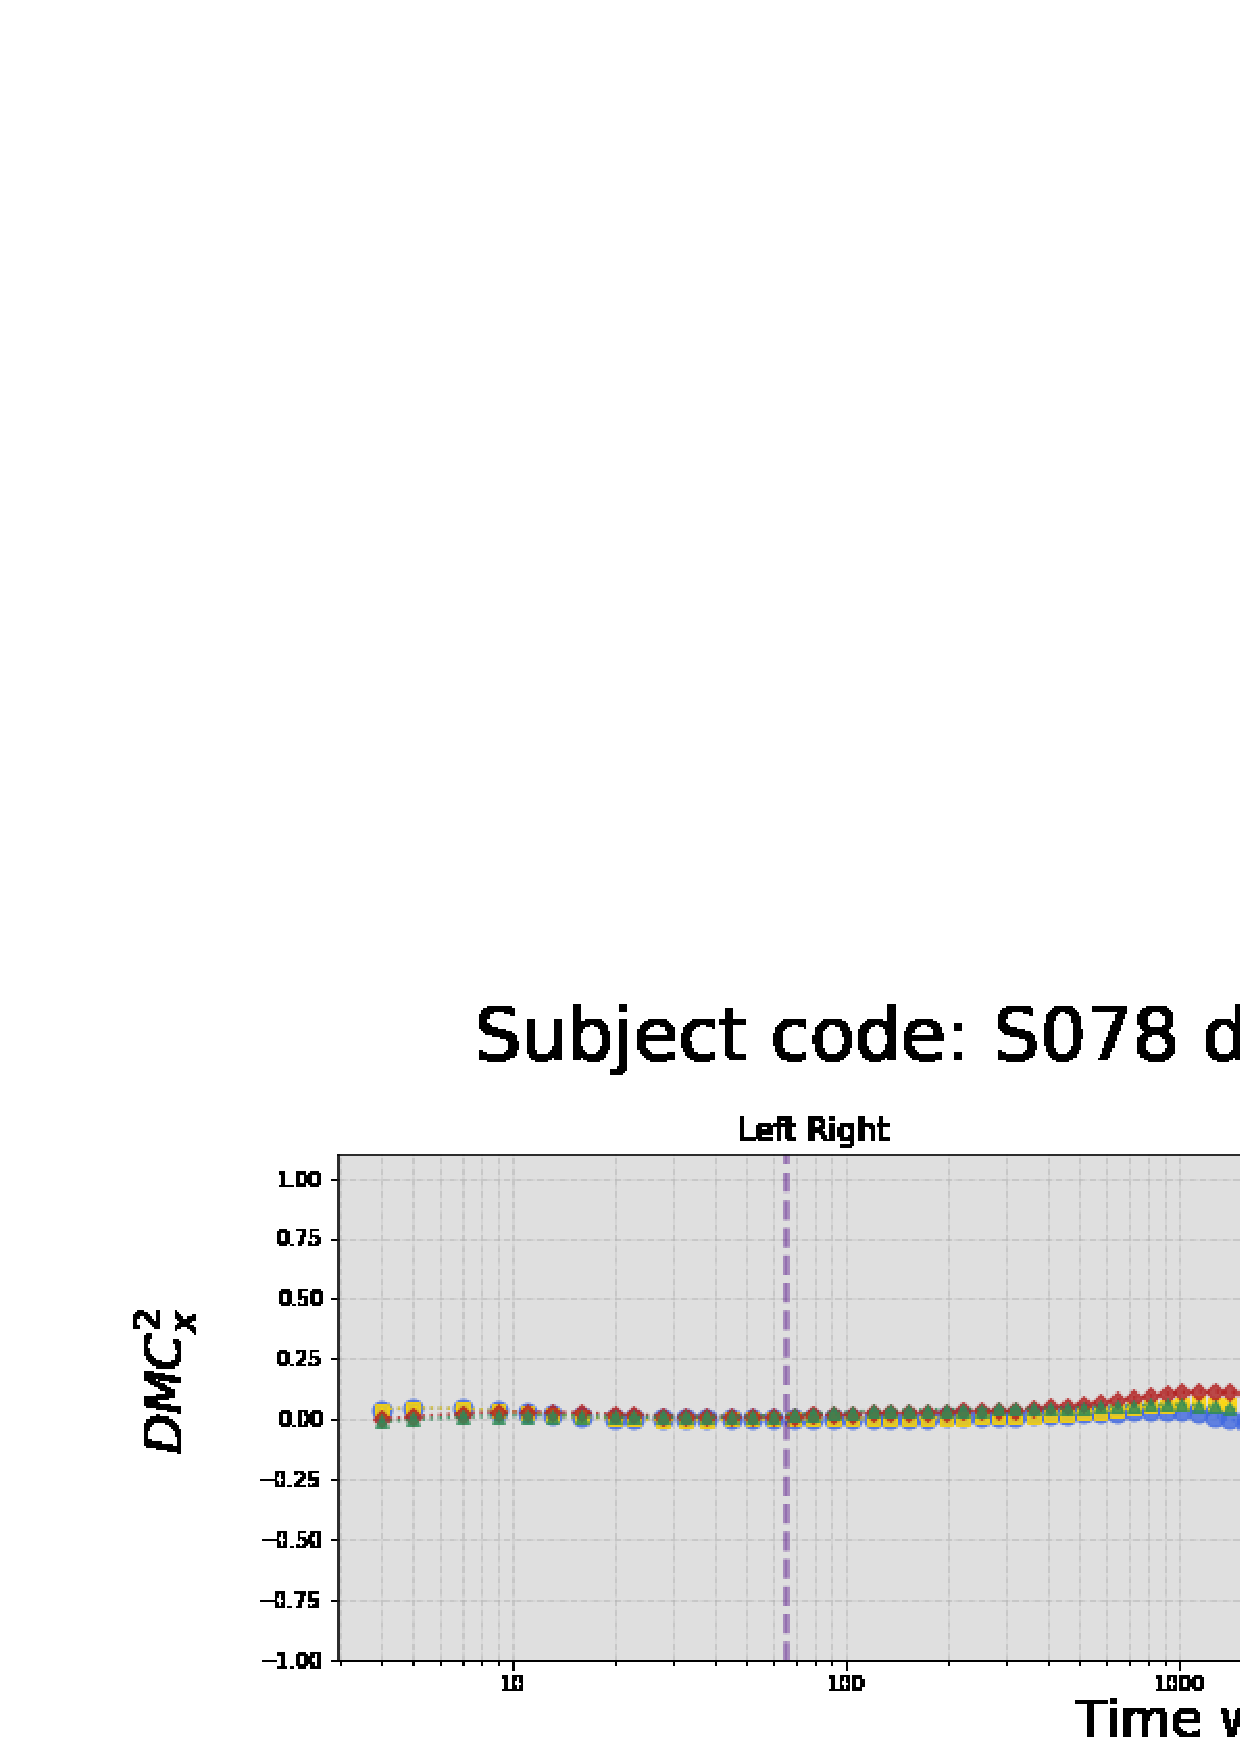
\includegraphics[width=.9\textwidth]{../output/figs/stats/S078.jpg}
      Figure caption text here, please use this space for the figure panel descriptions instead of using subfigure commands. A: Lorem ipsum dolor sit amet. B: Consectetur adipiscing elit.}
    \label{fig78}
\end{figure}

\begin{figure}[!h]
    \caption{{\bf Bold the figure title.}
    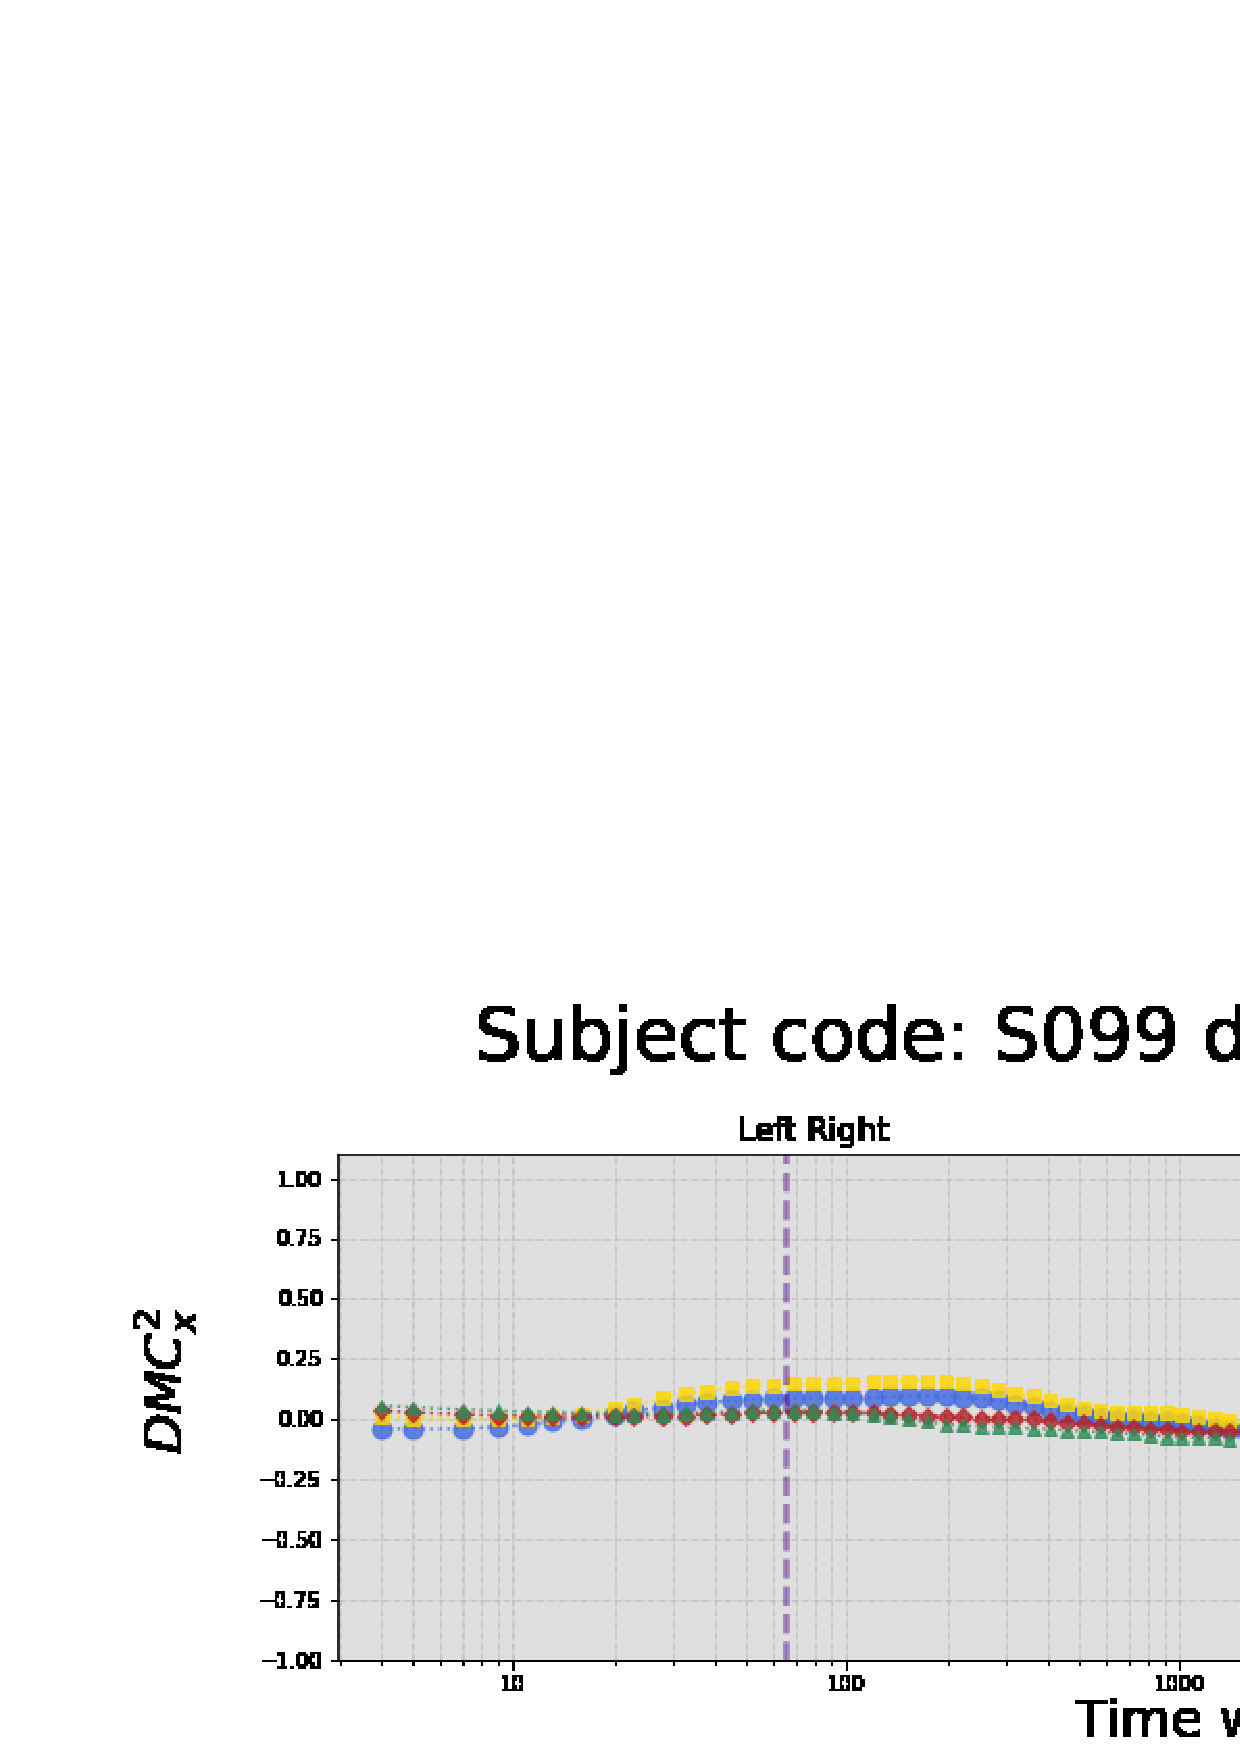
\includegraphics[width=.9\textwidth]{../output/figs/stats/S099.jpg}
      Figure caption text here, please use this space for the figure panel descriptions instead of using subfigure commands. A: Lorem ipsum dolor sit amet. B: Consectetur adipiscing elit.}
    \label{fig99}
\end{figure}


\begin{figure}[!h]
    \caption{{\bf Bold the figure title.}
    \includegraphics[width=.9\textwidth]{../output/figs/global/mean.jpg}
      Figure caption text here, please use this space for the figure panel descriptions instead of using subfigure commands. A: Lorem ipsum dolor sit amet. B: Consectetur adipiscing elit.}
      \label{glob_mean}
\end{figure}



\begin{figure}[!h]
    \caption{{\bf Bold the figure title.}
    \includegraphics[width=.9\textwidth]{../output/figs/global/median.jpg}
      Figure caption text here, please use this space for the figure panel descriptions instead of using subfigure commands. A: Lorem ipsum dolor sit amet. B: Consectetur adipiscing elit.}
    \label{glob_median}
\end{figure}

\begin{figure}[!h]
    \caption{{\bf Bold the figure title.}
    \includegraphics[width=.9\textwidth]{../output/figs/global/std pop.jpg}
    Figure caption text here, please use this space for the figure panel descriptions instead of using subfigure commands. A: Lorem ipsum dolor sit amet. B: Consectetur adipiscing elit.}
    \label{glob_std_pop}
\end{figure}

Nulla mi mi, venenatis sed ipsum varius, Table~\ref{table1} volutpat euismod diam. Proin rutrum vel massa non gravida. Quisque tempor sem et dignissim rutrum. Lorem ipsum dolor sit amet, consectetur adipiscing elit. Morbi at justo vitae nulla elementum commodo eu id massa. In vitae diam ac augue semper tincidunt eu ut eros. Fusce fringilla erat porttitor lectus cursus, vel sagittis arcu lobortis. Aliquam in enim semper, aliquam massa id, cursus neque. Praesent faucibus semper libero.

%PLOS does not support heading levels beyond the 3rd (no 4th level headings).
\subsection*{\lorem\ and \ipsum\ nunc blandit a tortor}
\subsubsection*{3rd level heading} 
Maecenas convallis mauris sit amet sem ultrices gravida. Etiam eget sapien nibh. Sed ac ipsum eget enim egestas ullamcorper nec euismod ligula. Curabitur fringilla pulvinar lectus consectetur pellentesque. Quisque augue sem, tincidunt sit amet feugiat eget, ullamcorper sed velit. Sed non aliquet felis. Lorem ipsum dolor sit amet, consectetur adipiscing elit. Mauris commodo justo ac dui pretium imperdiet. Sed suscipit iaculis mi at feugiat. 

\begin{enumerate}
	\item{react}
	\item{diffuse free particles}
	\item{increment time by dt and go to 1}
\end{enumerate}


\subsection*{Sed ac quam id nisi malesuada congue}

Nulla mi mi, venenatis sed ipsum varius, volutpat euismod diam. Proin rutrum vel massa non gravida. Quisque tempor sem et dignissim rutrum. Lorem ipsum dolor sit amet, consectetur adipiscing elit. Morbi at justo vitae nulla elementum commodo eu id massa. In vitae diam ac augue semper tincidunt eu ut eros. Fusce fringilla erat porttitor lectus cursus, vel sagittis arcu lobortis. Aliquam in enim semper, aliquam massa id, cursus neque. Praesent faucibus semper libero.

\begin{itemize}
	\item First bulleted item.
	\item Second bulleted item.
	\item Third bulleted item.
\end{itemize}

\section*{Discussion}
Nulla mi mi, venenatis sed ipsum varius, Table~\ref{table1} volutpat euismod diam. Proin rutrum vel massa non gravida. Quisque tempor sem et dignissim rutrum. Lorem ipsum dolor sit amet, consectetur adipiscing elit. Morbi at justo vitae nulla elementum commodo eu id massa. In vitae diam ac augue semper tincidunt eu ut eros. Fusce fringilla erat porttitor lectus cursus, vel sagittis arcu lobortis. Aliquam in enim semper, aliquam massa id, cursus neque. Praesent faucibus semper libero.

\section*{Conclusion}

CO\textsubscript{2} Maecenas convallis mauris sit amet sem ultrices gravida. Etiam eget sapien nibh. Sed ac ipsum eget enim egestas ullamcorper nec euismod ligula. Curabitur fringilla pulvinar lectus consectetur pellentesque. Quisque augue sem, tincidunt sit amet feugiat eget, ullamcorper sed velit. 

Sed non aliquet felis. Lorem ipsum dolor sit amet, consectetur adipiscing elit. Mauris commodo justo ac dui pretium imperdiet. Sed suscipit iaculis mi at feugiat. Ut neque ipsum, luctus id lacus ut, laoreet scelerisque urna. Phasellus venenatis, tortor nec vestibulum mattis, massa tortor interdum felis, nec pellentesque metus tortor nec nisl. Ut ornare mauris tellus, vel dapibus arcu suscipit sed. Nam condimentum sem eget mollis euismod. Nullam dui urna, gravida venenatis dui et, tincidunt sodales ex. Nunc est dui, sodales sed mauris nec, auctor sagittis leo. Aliquam tincidunt, ex in facilisis elementum, libero lectus luctus est, non vulputate nisl augue at dolor. For more information, see.

\section*{Supporting information}

% Include only the SI item label in the paragraph heading. Use the \nameref{label} command to cite SI items in the text.
\paragraph*{S1 Fig.}
\label{S1_Fig}
{\bf Bold the title sentence.} Add descriptive text after the title of the item (optional).

\paragraph*{S2 Fig.}
\label{S2_Fig}
{\bf Lorem ipsum.} Maecenas convallis mauris sit amet sem ultrices gravida. Etiam eget sapien nibh. Sed ac ipsum eget enim egestas ullamcorper nec euismod ligula. Curabitur fringilla pulvinar lectus consectetur pellentesque.

\paragraph*{S1 File.}
\label{S1_File}
{\bf Lorem ipsum.}  Maecenas convallis mauris sit amet sem ultrices gravida. Etiam eget sapien nibh. Sed ac ipsum eget enim egestas ullamcorper nec euismod ligula. Curabitur fringilla pulvinar lectus consectetur pellentesque.

\paragraph*{S1 Video.}
\label{S1_Video}
{\bf Lorem ipsum.}  Maecenas convallis mauris sit amet sem ultrices gravida. Etiam eget sapien nibh. Sed ac ipsum eget enim egestas ullamcorper nec euismod ligula. Curabitur fringilla pulvinar lectus consectetur pellentesque.

\paragraph*{S1 Appendix.}
\label{S1_Appendix}
{\bf Lorem ipsum.} Maecenas convallis mauris sit amet sem ultrices gravida. Etiam eget sapien nibh. Sed ac ipsum eget enim egestas ullamcorper nec euismod ligula. Curabitur fringilla pulvinar lectus consectetur pellentesque.

\paragraph*{S1 Table.}
\label{S1_Table}
{\bf Lorem ipsum.} Maecenas convallis mauris sit amet sem ultrices gravida. Etiam eget sapien nibh. Sed ac ipsum eget enim egestas ullamcorper nec euismod ligula. Curabitur fringilla pulvinar lectus consectetur pellentesque.

\section*{Acknowledgments}
Cras egestas velit mauris, eu mollis turpis pellentesque sit amet. Interdum et malesuada fames ac ante ipsum primis in faucibus. Nam id pretium nisi. Sed ac quam id nisi malesuada congue. Sed interdum aliquet augue, at pellentesque quam rhoncus vitae.



% Either type in your references using
% \begin{thebibliography}{}
% \bibitem{}
% Text
% \end{thebibliography}
%
% or
%
% Compile your BiBTeX database using our plos2015.bst
% style file and paste the contents of your .bbl file
% here. See http://journals.plos.org/plosone/s/latex for 
% step-by-step instructions.
% 


\bibliography{../bibtex/zotero_exp_22_12_16.bib}


\end{document}

